\chapter{绪论}
\section{研究背景以及问题提出}
\subsection{亚临界转捩与槽道湍流带}
湍流是指流体运动中出现的一种不规则、混乱的运动状态,是与流动结构规律简单的层流相对的流动现象。与稳定的层流流动不同,湍流具有很强的随机性和非线性,流场中的速度场、压力场、密度分布等物理量都会不断发生变化和波动。湍流现象广泛存在于自然界和工业领域中,大部分的流体如水流、气流等都可能产生湍流,研究湍流形成的机理有很强的现实意义和理论意义。在工程上,湍流对飞行器和船舶设计都有着重要的影响:在飞行器设计中,湍流的存在会引起飞行器表面的阻力、升力和气动特性等方面的变化,从而影响飞行器的性能和稳定性;在船舶设计中,湍流的影响主要表现在水动力方面。湍流会引起船体表面的阻力和摩擦,从而增加燃油消耗和减缓船速。设计师一般通过优化外形减小湍流生成概率,即尽量使流动接近稳定规律的层流状态,而深入理解湍流的生成机制有助于更进一步达到这一目的。

在研究湍流的生成和控制的研究领域中,湍流转捩是一种流体运动中的重要现象,它指的是流动从稳定流动状态转变为不稳定湍流状态的过程。对湍流转捩机理认识的加深有助于更进一步的控制湍流的生成与强度。湍流转捩的机理十分复杂,它受到多种因素的影响,且在转捩过程中存在强烈的非线性现象和多尺度效应。目前,研究湍流转捩现象的方法主要包括实验、数值模拟和理论分析三种。其中实验方法是研究湍流转捩最直接的手段,通过在实验室中建立不同几何形状的流动系统,可以观察和测量湍流转捩现象的发生和特性。例如,可以利用热线或压力传感器等测量设备来检测流动中的湍流现象和变化。然而,实验方法往往需要消耗大量的时间和成本,且在实验中很难对流场进行直接控制。

理论分析方法主要是基于数学和物理学原理,通过推导数学公式和解析式,来研究流动的发生和演化过程。理论分析方法可以提供对湍流转捩机理的深入理解和阐释,同时也可以为实验和数值模拟提供基础和指导。理论分析方法往往需要对流体的运动方程、控制方程和边界条件等进行精细的推导和处理,因此需要高超的数学和物理学知识。

数值模拟是另一种研究湍流转捩现象的常用方法。数值模拟是通过建立数学模型和计算方法,对流体的运动和相应的物理量进行模拟和计算。数值模拟方法可以对流动的各种物理量进行精细的模拟和分析,同时也可以通过对流场的控制变量进行调整,研究湍流转捩的发生条件和机理。数值模拟方法通常需要一定的计算资源和复杂的算法,但是在研究湍流转捩现象时,它可以提供更为详尽的信息和更好的可控性,因此在实际应用中也得到了广泛的使用。同时这也是本文中研究湍流转捩的主要实验方法。

仅受法向固壁限制下的槽道流动(泊肃叶流动,即在流向和展向上无穷大,法向上有固壁限制的流动模型)是研究湍流转捩的理想流动模型之一。Orszag等人通过数值计算证明,当雷诺数大于临界值$Re_cr = 5772$时泊肃叶流会因为流场中的微小扰动造成线性失稳进而导致流场从层流转化为湍流,此时转捩现象是由线性不稳定因素\cite{orszag_1971}主导的。但事实上在雷诺数远低于这个临界值的情况下,槽道流中也能观察到湍流转捩现象。Tsukahara等人通过数值模拟足够大槽道中的泊肃叶流动发现了局部湍流转捩现象\cite{Tsukahara2005DNSOT}(见图\ref{fig:2005band}),更具体地说是一种由交替的高低速速度条纹聚合而成的局部带状湍流。从整体上看带状湍流与主流方向呈一定的倾角,带与带之间互相平行并由接近层流的低湍流度区域分隔开来。此时雷诺数为$Re = 1546$远低于前文提到的线性失稳临界值($Re_{cr} = 5772$),这表明主导转捩的是非线性因素。称这种现象为亚临界转捩,这种特殊的带状湍流结构则被称为湍流带。

\begin{figure}[H]
	\subfigbottomskip = 2pt
	%\subfigcapskip=-5pt
	\begin{minipage}[h]{\linewidth}
	\centering
	\subfigure{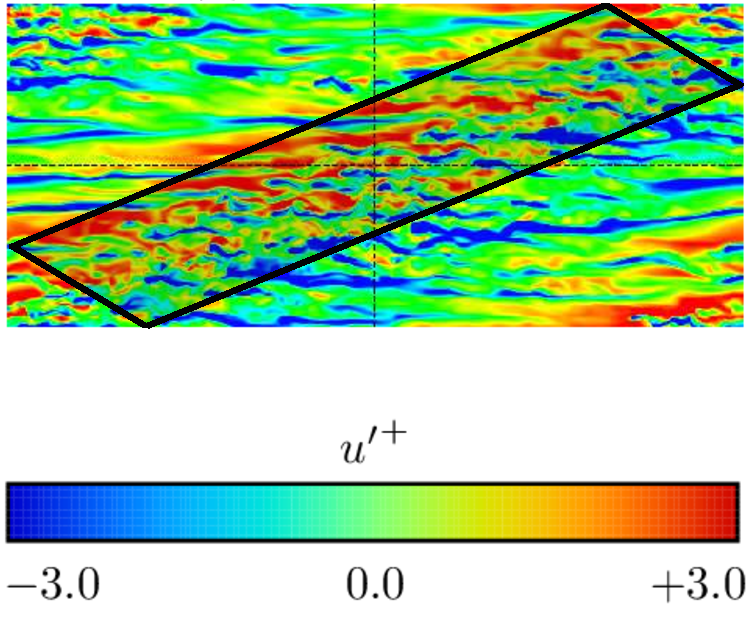
\includegraphics[width = 0.5\textwidth]{figures/intro/tsukahara.pdf}}
	\end{minipage}
	\quad
	\caption{低雷诺数下足够大槽道中的局部化湍流结构\cite{Tsukahara2005DNSOT}。主流方向为从左到右(周期性边界条件),雷诺数为$Re_m = 2320$。图中展示的是x-z截面上流向脉动速度$u‘$的分布。黑框部分可以观察到由高低速速度条纹组成的局部高湍流度区域,黑框之外的是低湍流度区域。也即是此时由于非线性因素产生了局部化的湍流结构。}
\label{fig:2005band}
\end{figure}

随后的研究\cite{TsukaharaKawaguchi2014, Tuckerman2014, Xiong2015, Tao2018, Kanazawa2018, Paranjape2019, Shimizu2019, Paranjape2020, Tuckerman2020, Liu2020, Duguet2020}进一步证实了槽道中湍流带的客观存在并讨论了相关力学特性。如图\ref{fig:2005band}所示展现的湍流带结构是在足够大计算域中模拟得到的,但该尺寸的计算域事实上仍未能完全展现出湍流带的完整结构;而在更大计算域中的湍流带模拟研究\cite{Xiong2015, Tao2018, Kanazawa2018, Paranjape2019, Shimizu2019}可以看到,湍流带具有有限的长度(不能无限生长延申),其结构总体上可以分为三个部分,分别是:活跃的下游端头,消散性的上游端头以及有限长度的由高低速度条纹交替组成的身体(图\ref{fig:num_band}(a)),且湍流带整体会以与主流方向呈一定倾角的方向在槽道中运动(即在展向和流向上都有速度分量,且流向速度分量与主流一致)。除了数值实验,物理实验中也观察到了带状局部湍流(\ref{fig:exp_band}),且与数值模拟结果相同湍流带具有相同的结构,如与主流呈一定的倾角,具有倾斜的运动速度,活跃的下游头部等。这进一步证明了湍流带是客观存在而不是由数值误差造成的。
\begin{figure}[htb]
	\subfigbottomskip = 2pt
	%\subfigcapskip=-5pt
	\begin{minipage}[h]{\linewidth}
	\centering
	\subfigure{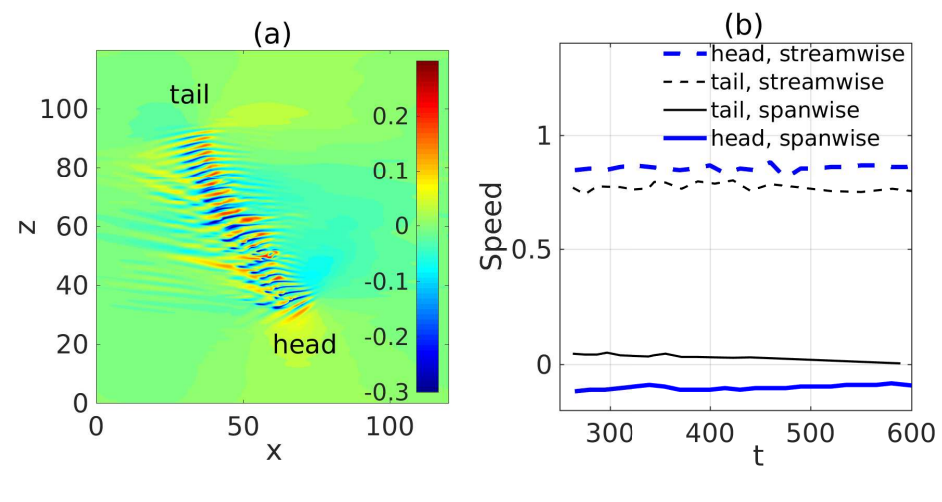
\includegraphics[width = 0.8\textwidth]{figures/intro/num_band.png}}
	\end{minipage}
	\quad
	\caption{中在$Re = 750$下数值模拟得到的单个湍流带,主流流向为从左到右\cite{Xiao2020}。(a)y=-0.5的x-z截面上流向脉动速度$u‘$的分布,可以看到单个相对于主流方向倾斜的湍流带。(b)湍流带的下游端头(头部,head)和上游端头(尾部,tail)附近的展向和流向速度分量随时间变化。}
\label{fig:num_band}
\end{figure}

\begin{figure}[H]
	\subfigbottomskip = 2pt
	%\subfigcapskip=-5pt
	\begin{minipage}[h]{\linewidth}
	\centering
	\subfigure{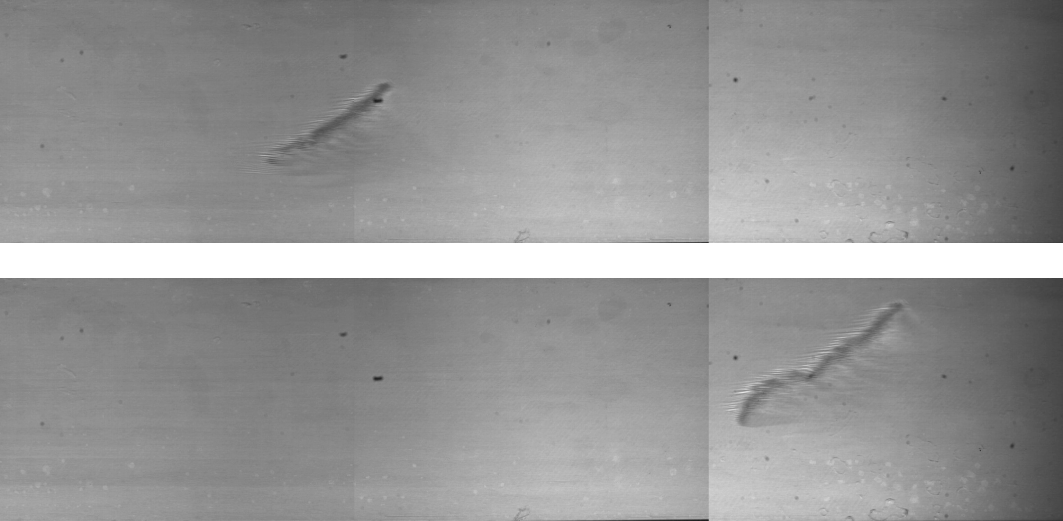
\includegraphics[width = 0.7\textwidth]{figures/intro/experimental_band.png}}
	\end{minipage}
	\quad
	\caption{在Re=700时,实际槽道实验中观察到的向下游运动生长的单个倾斜湍流带。主流方向为从左向右,其中添加了反光云母颗粒进行可视化\cite{Paranjape2020}。可以观察到与数值实验中一致的头部,尾部,以及倾斜运动。}
\label{fig:exp_band}
\end{figure}

值得注意的一点是,最近的研究表明湍流带活跃的下游端头对湍流带的整体自持起到关键性的作用。部分研究\cite{Kanazawa2018, Paranjape2019, Shimizu2019, Xiao2020}进一步认为低雷诺数下,湍流带的运动主要是由下游端头所主导的。过去的许多研究表明,湍流带主体的湍流结构是从下游端头处不断生成的(图\ref{fig:band_generation}),且在低雷诺数下下游端头决定了湍流带的生长机制\cite{Paranjape2019, Shimizu2019, Xiao2020, Song2020, Liu2020}。根据实际测量可以发现,下游端头在流向和展向上存在一个自身的运动速度,且该运动速度与湍流带主体的运动速度有明显的速度差,这种速度差异决定了湍流带与主流方向的倾角大小\cite{Xiao2020b}。关于下游端头运动速度的大小,展向速度分量大小约为0.1(以层流时抛物线速度型的中心流速为基本单位)且在不同雷诺数下基本不变(图\ref{fig:num_band}(b))。同时,下游端头的展向速度与湍流带整体关于流向的倾角也是互相关联的\cite{Paranjape2019,Shimizu2019,Xiao2020}(即如果湍流带关于流向的倾角相反,则下游端头的展向速度方向也是相反的)。

\begin{figure}[htb]
	\subfigbottomskip = 2pt
	%\subfigcapskip=-5pt
	\begin{minipage}[h]{\linewidth}
	\centering
	\subfigure{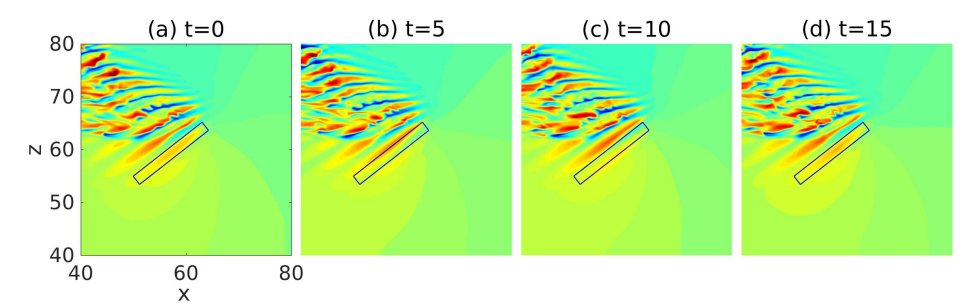
\includegraphics[width = \textwidth]{figures/intro/band_generation.png}}
	\end{minipage}
	\quad
	\caption{文献\cite{Xiao2020}中提到的湍流带条纹生成机制。交替的高低速条纹形成的波状结构自头部匀速生成。}
\label{fig:band_generation}
\end{figure}

Shimizu\& Manneville 进一步研究了更大的计算域中多湍流带相互作用的行为\cite{Shimizu2019}。他们发现从随着雷诺数的不断升高湍流带的带状特征会逐步减少直到雷诺数大于950,此时湍流带展向宽度开始扩大并开始生成更多扩散性的湍流。此外在这个过程中,湍流带自身会出现频繁地分裂,分岔现象,带与带之间开始出现相互作用(图\ref{fig:Re_band})(这些行为在低雷诺数下也能观察到,但频率极低)。但即便如此仍能观察到湍流带的下游端头表现出很强的一致性。
\begin{figure}[htb]
	\subfigbottomskip = 2pt
	%\subfigcapskip=-5pt
	\begin{minipage}[h]{\linewidth}
	\centering
	\subfigure{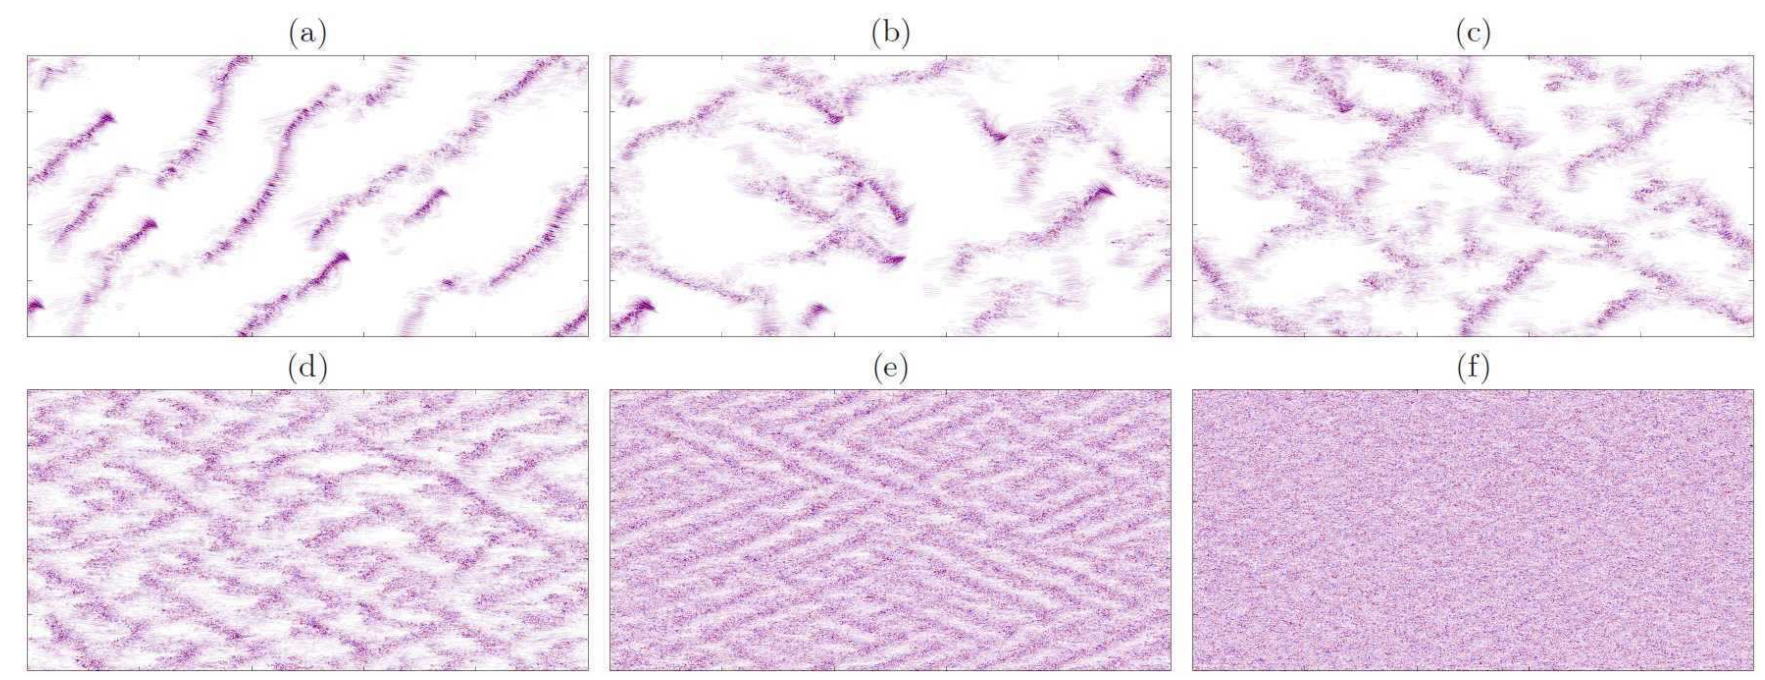
\includegraphics[width = 1\textwidth]{figures/intro/Re_band.png}}
	\end{minipage}
	\quad
	\caption{大计算域内多湍流带的集体行为模式随雷诺数升高的变化\cite{Shimizu2019}。(a)Re = 850:计算域中所有湍流带的运动方向基本相同;(b)Re = 1050:部分湍流带开始出现分裂行为,分裂出的湍流带在展向上以相反方向运动;(c)Re = 1200:分裂持续进行且湍流带宽度开始增大;(d) Re = 1800:带间相互作用逐渐成为主导 (e) Re = 3000: 形成稳定的双向带状湍斑 (f) Re = 4000: 湍流基本充满整个流域,基本观察不到湍流带结构。 }
\label{fig:Re_band}
\end{figure}
上述研究中都以平板泊肃叶流动作为基础模型(周期槽道或者无限长槽道)深入研究了湍流带的性质,这在数值计算和理论分析上有很大的便利。但在实际物理实验中并不存在边界无穷大的实体模型,此时不可避免地要考虑展向上侧壁效应的存在。前文提到,湍流带下游头部在展向上存在一个接近恒定的速度分量(约为0.1),因此可以预见的是,如果湍流带没有因为外力影响或者带间作用消失的话,单个湍流带的头部在经过足够长的时间后必然会与侧壁发生碰撞,且侧壁的约束作用必然会对侧壁附近的湍流形态会产生影响。现有研究详细讨论了平板泊肃叶流动模型下湍流带带间的相互作用以及由此生成的流动模式。但大部分主要关注的是远离壁面的湍流现象,关于湍流带与侧壁的相互作用尚未引起足够的注意。Takeishi等人研究了槽道宽高比对转捩现象的影响\cite{Takeishi2015},但其仅考虑了最大宽高比为9的情况,这种情况下槽道的宽度不足以让湍流带完全发展出能稳定自持的下游端头,也就无法研究湍流带端头与侧壁碰撞后的真实情况。由于湍流带头部的展向运动速度不大,湍流带需要一定的时间才能靠近侧壁。因此对于关注湍流带短期行为的研究来说,侧壁效应的影响很小。

目前为止,明确讨论侧壁效应对湍流带影响的文献为\cite{Paranjape2019},作者在物理实验中观察到低雷诺数下湍流带在下游头部与槽道侧壁碰撞后快速衰减消失。Takeishi等人的工作提出在宽高比大于4的槽道中边壁效应通过消减附近的涡结构导致了展向局部湍斑\cite{Takeishi2015},然而文中并没有探讨湍流带碰壁后存活与否的临界雷诺数。因此,本论文第三章的研究目的就是为了确定该临界雷诺数以及可能的潜在机制。所得结论能对将来类似的物理实验提供了一定的参考作用。

\subsection{湍流带自持性和瞬态性}
前文描述了低雷诺数下槽道流动中存在的局部湍流现象,在同样的剪切流动如圆管流动、库埃特流等经典流动模型中,同样也观察到了低雷诺数下的局部湍流现象\cite{Hof2006FiniteLO,Barkley2016}。已有研究证明,转捩雷诺数下管流和圆管流动中的局部湍流存在所谓的瞬态性\cite{Barkley2016}。如图\ref{fig:lifetime}所示,在雷诺数相对较低时湍流带在发展有限长的时间后会消散(即具有有限的寿命);当雷诺较高时湍流带在发展足够长的时间后则会产生分裂。统计多个局部湍流的寿命能进一步得出圆管中局部湍流的寿命服从一个关于雷诺数的分布(图\ref{fig:lifetime})\cite{Sabine1998}。后续的研究\cite{Barkley2016,POMEAU19863,Lemoult2016DirectedPP}针对圆管局部湍流分裂或消失的特性,尝试用逾渗(Directed Percolation,DP)模型尝试解释圆管流场中局部湍流的群体行为,取得了一定的成果。

\begin{figure}[H]
	\subfigbottomskip = 2pt
	%\subfigcapskip=-5pt
	\begin{minipage}[h]{\linewidth}
	\centering
	\subfigure{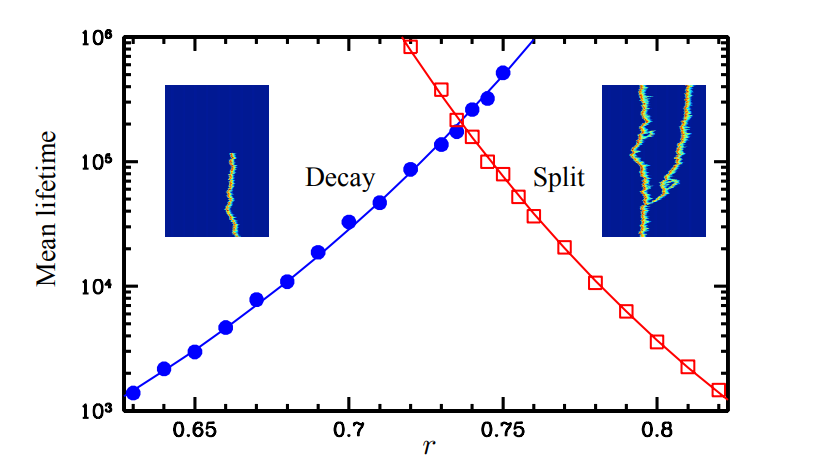
\includegraphics[width = 0.75\textwidth]{figures/intro/lifetime_split.png}}
	\end{minipage}
	\quad
	\caption{管道流动局部湍流的寿命分布\cite{Barkley2016}。横轴是雷诺数,纵轴是平均寿命。在雷诺数小于某个值时,管道湍流在运行一定时间后会消失;反之则会分裂。}
\label{fig:lifetime}
\end{figure}

低雷诺数下圆管流和库埃特流中局部转捩湍流的瞬态性已被验证,可以合理地期望在低雷诺数下同样作为剪切流的槽道流中的局部湍流(即湍流带)也应具有瞬态性(有限寿命)。但已有的研究认为有别于另外两种剪切流动,在雷诺数约为$Re_{cr} \simeq 650-660$时槽道湍流带是永久自持的而不是瞬态的,即湍流带能一直存活不会消失\cite{Kanazawa2018,Tao2018,Paranjape2019}。该雷诺数远低于基于DP理论预测的湍流带可自持的临界雷诺数$Re_{cr,DP}$\cite{Sano2016}。然而最近的一项工作表明,低雷诺数下长度受控的湍流带本质上仍是瞬态的而不是自持的\cite{xu_song_2022}。作者基于直接数值模拟方法观察了Re = 655情况下单个湍流带的发展情况,发现在经过极长的一段的时间后,湍流带的下游头部部分会突然自行消失(图\ref{fig:decay_KE})。前文提到在低雷诺数下湍流带的头部对湍流带整体的存在和条纹生成起到了至关重要的作用,头部的瞬态性意味着此时湍流带整体也是瞬态的,只是寿命远超过去设想的长度($T \simeq O(10^5)$)。值得注意的是根据文中的结论是基于单个长度受数值控制的湍流带,关于更高雷诺数下无长度限制的湍流带的寿命分布以及是否表现出瞬态性等问题仍是开放的。作者指出基于已有研究更高雷诺数下湍流带的整体大小和寿命长度将会急剧增大,直接数值模拟湍流带的整个演化过程将会需要巨大空间尺度和时间尺度。若继续采用文中的直接数值模拟方法则其计算成本和时间成本将是难以承受的。因此亟需一种计算成本更低的方法,可以对湍流带的宏观发展作出一定可靠的预测,并能由此进一步得到湍流带的寿命分布。

\begin{figure}[htb]
	\subfigbottomskip = 2pt
	%\subfigcapskip=-5pt
	\begin{minipage}[h]{\linewidth}
	\centering
	\subfigure{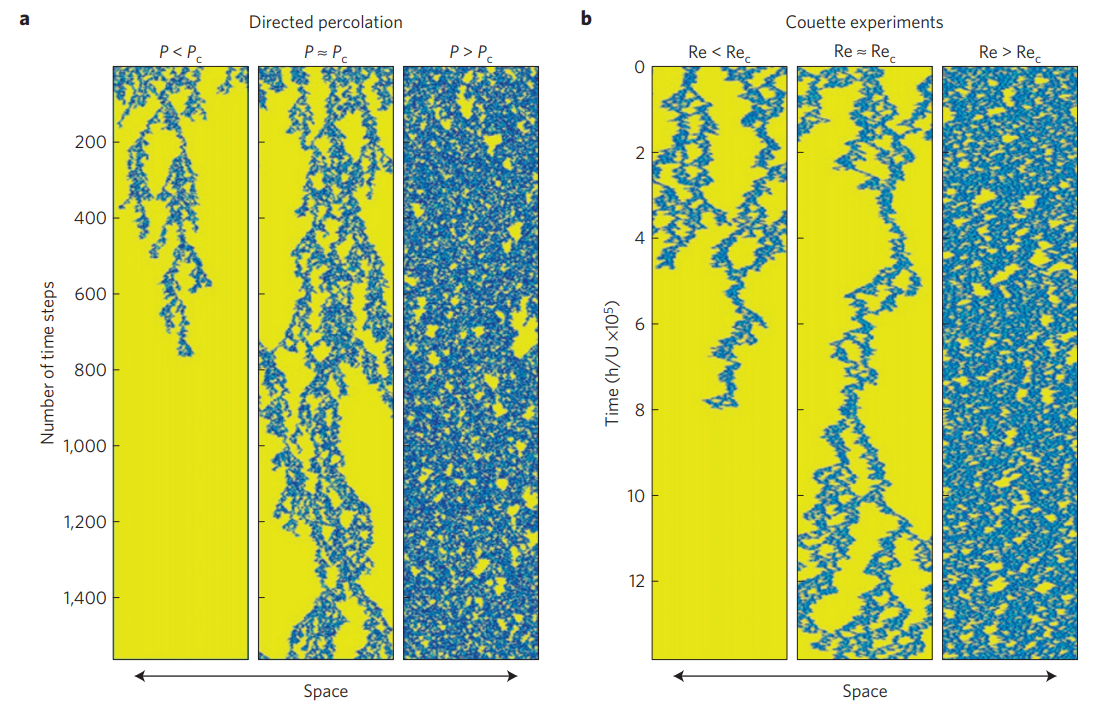
\includegraphics[width = 1\textwidth]{figures/intro/DP.png}}
	\end{minipage}
	\quad
	\caption{文献\cite{Lemoult2016DirectedPP}中关于DP与湍流分裂行为的共性对比。(a)链接概率高于、等于、低于临界值$P_c$定向渗流模拟。这里,活性位点以蓝色显示,吸收态以黄色显示。在临界点以下,所有位点最终进入吸收态(左图)。在接近临界点(中间面板)时,活性位点持续存在,但出现了大的层流区域(尺度不变性)。最后,对于P>Pc(右侧面板),活性位点占据了域的很大一部分。(b)Couette流动(管流)的时空图,小于、等于和高于临界雷诺数。某一时刻上的水平线对应的是该时刻实验中流场的截面流场(层流区域以黄色显示,湍流区域以蓝色示出)。在雷诺数小于临界值时(左侧),湍流在足够长的时间后消失。在临界值附近(中间)湍流能自持,但只占据了该领域的一小部分;雷诺数远高于临界值(右图),局部湍流斑块占据了流动域的大部分}
\label{fig:DP}
\end{figure}

\begin{figure}[H]
	\subfigbottomskip = 2pt
	%\subfigcapskip=-5pt
	\begin{minipage}[h]{\linewidth}
	\centering
	\subfigure{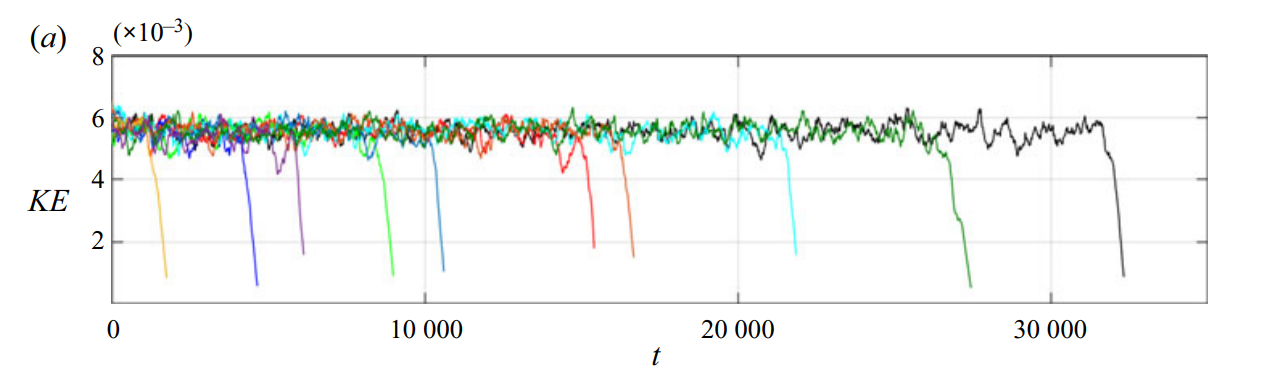
\includegraphics[width = 1\textwidth]{figures/intro/decay_KE.png}}
	\end{minipage}
	\quad
	\caption{文献\cite{xu_song_2022}关于湍流带发展的流场能量随时间变化图,横轴是时间纵轴是流场能量,作者通过一定的数值手段仅关注湍流带的头部附近流场。文章针对同一个初始湍流带运行了10次,获得了十根不同的能量变化图线。可以看到最终能量都会迅速衰减到一个极小值,这说明湍流带的头部在运行一段时间后最终衰减消失(层流化)。}
\label{fig:decay_KE}
\end{figure}

本文注意到,Anton等人基于一种简化神经网络预测了另一种简化剪切流MFE流动\cite{MFE}的瞬态性\cite{Anton2023}。MFE流动的湍流与湍流带相似,流场在长期处于湍流状态后会在某一时间点突然变为层流状态。如图\ref{fig:MFE_decay}所示,初始时流场处于湍流状态,能量较低;当流场突然层流化时能量也会陡升至某一水平不再下降。可以认为MFE流动的湍流也具有有限的寿命,且通过多次重复实验可知该寿命也服从于某个关于雷诺数的分布。该文作者声称他们构造的神经网络成功预测MFE流动的突然层流化(即瞬态性),并基于完成训练的神经网络的预测结果得到了与理论高度吻合的MFE湍流的寿命关于雷诺数的分布。众所周知神经网络的计算成本主要集中在前期训练阶段,当训练完成后网络预测所需的算力消耗极低(与直接数值模拟相比)。受该工作启发,本文尝试将该文提到的预测方法迁移到湍流带的瞬态性预测上。在对该方法做了一系列适当合理的修改后,本文得到了一些值得注意的结果。

\begin{figure}[H]
	\subfigbottomskip = 2pt
	%\subfigcapskip=-5pt
	\begin{minipage}[h]{0.54\linewidth}
	\centering
	\subfigure[]{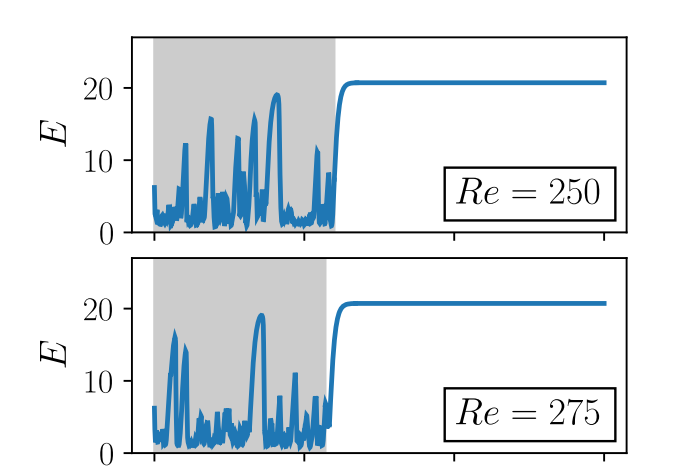
\includegraphics[width = 0.75\textwidth]{figures/intro/MFE_E.png}}
	\end{minipage}
	\quad
	\begin{minipage}[h]{0.45\linewidth}
	\centering
	\subfigure[]{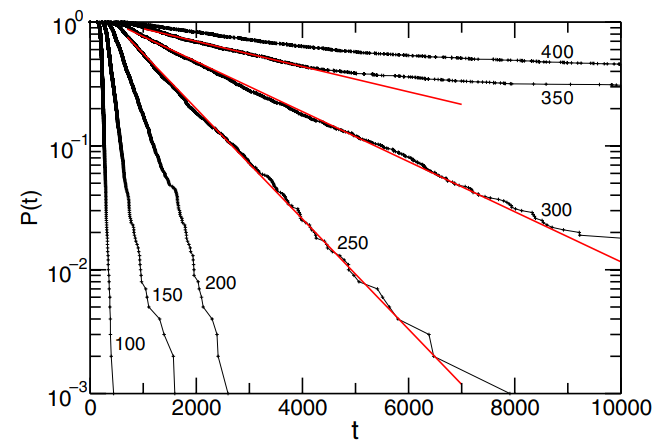
\includegraphics[width = 1\textwidth]{figures/intro/MFE_time.png}}
	\end{minipage}
	\quad
	\caption{(a)不同雷诺数下MFE流动的流场能量随时间的大致变化\cite{Anton2023},横轴是时间,纵轴是流场能量。(b)MFE流动的湍流存活率随时间的关系。}
\label{fig:MFE_decay}
\end{figure}

%\section{文献综述}
%在亚临界转捩雷诺数下,足够大的槽道中会出现局部带状湍流结构,即所谓的湍流带 \cite{Tsukahara2005, TsukaharaKawaguchi2014, Tuckerman2014, Xiong2015, Tao2018, Kanazawa2018, Paranjape2019, Shimizu2019, Paranjape2020, Xiao2020, Tuckerman2020, Liu2020, Duguet2020}。我们可以观察到,槽道中形成的湍流带会以与主要流动(定压力梯度驱动或定流量驱动)方向呈一定倾角,且会在槽道中漂移、发展。从湍流带的整体上看,充分发展后的湍流带可以分为三个部分:一个活跃的下游端头,一个呈现消散性的上游端头,以及中间由速度条纹组成的有限长度的身体\cite{Xiong2015, Tao2018, Kanazawa2018, Paranjape2019, Shimizu2019}。需要注意的一点是,最近的研究表明湍流带活跃的下游端头对湍流带的整体自持起到关键性的作用,某些研究\cite{Kanazawa2018, Paranjape2019, Shimizu2019, Xiao2020}甚至认为在低雷诺数下,湍流带的漂移行为主要是由下游端头所驱动的。过去的许多研究表明,湍流带中的湍流结构是由下游端头不断生成的。且在低雷诺数下,下游端头决定了湍流带的生长机制\cite{Paranjape2019, Shimizu2019, Xiao2020, Song2020, Liu2020}。根据实际测量可以发现,下游端头在流向和展向上存在自身的漂移速度,且端头的漂移速度与湍流带主体的漂移速度有明显的速度差,且这种速度差异决定了湍流带与主流方向的倾角大小\cite{Xiao2020b}。关于漂移速度的大小,展向上的速度分量基本不变大小约为0.1(以层流时抛物线速度型的中心流速为基本单位)。下游端头的展向速度与湍流带整体关于流向的倾角也是互相关联的\cite{Paranjape2019,Shimizu2019,Xiao2020}(即如果湍流带关于流向的倾角相反,则下游端头的展向速度方向也是相反的)。已有研究发现湍流带可以在雷诺数(基于半槽高以及抛物线速度型的中心流速)低至660左右自持。随着雷诺数的上升,湍流带的带状特征会逐步减少直到雷诺数大于950,此时湍流带开始在流向上变宽,更多扩散性的湍流开始产生。除此之外,湍流带自身开始频繁地分裂,分岔,带与带之间开始出现相互作用(在低雷诺数下也有类似的情况,但频率极低)。即便如此,湍流带的下游端头仍然表现出很强的鲁棒性。

%%在理论研究中,平板泊肃叶流动是研究无侧壁槽道中湍流产生的理想模型。但在实际物理实验中,我们不可避免地要考虑侧壁的存在。如前文所说,湍流带由于在展向上存在速度分量,我们可以预见在没有自行消失或者与其他湍流带相互作用的情况下,湍流带在一定时间内必然会与侧壁发生碰撞,且侧壁的约束作用必然会对侧壁附近的湍流形态会产生影响。

%已有的研究详细讨论了平板泊肃叶流动模型下湍流带带间的相互作用以及由此生成的流动模式。但目前为止相关研究主要关注远离避免的湍流现象,关于湍流带与侧壁的相互作用尚未引起足够的注意。在\cite{Takeishi2015}中研究了槽道宽高比对转捩现象的影响,但作者仅考虑了最大宽高比为9的情况,这种情况下槽道的宽度不足以让湍流带完全发展出能稳定自持的下游端头,也就无法研究湍流带端头与侧壁碰撞后的真实情况。由于湍流带头部的展向漂移速度不大(接近0.1),湍流带需要一定的时间才能靠近侧壁。因此对于关注湍流带短期行为的研究来说,侧壁效应的影响很小。例如某些尝试建立直接渗流相变理论和亚临界转捩的关系的物理实验\cite{Sano2016}。

%具我们所知,目前唯一明确讨论侧壁效应问题的文献为\cite{Paranjape2019}。作者在物理实验中观察到低雷诺数下湍流带在下游头部与槽道侧壁碰撞后快速衰减消失,然而侧壁效应同样。文献\cite{Takeishi2015}中提到宽高比大于4的槽道中,边壁效应通过消减附近的涡结构导致了展向局部湍斑。然而文中并没有提到湍流带在高于某个雷诺数的情况下能够在与边壁碰撞后存活,且湍流带消失的潜在机制也未被进一步讨论。因此,本文中第三部分的研究目的就是为了确定该临界雷诺数以及可能的潜在机制。所得结论能对将来类似的物理实验提供了一定的参考作用。

%在有壁面限制的剪切流动中,局部化湍流在亚临界转捩为湍流的过程中普遍存在。事实证明局部化湍流的本质上是随机瞬态的,在典型剪切流(如管道流和Couette流)中局部湍流可以存活极长的时间,并在某一时刻经过无记忆性衰减过程后突然层流化消失。这种瞬态性(与随机无记忆分裂作用一起)是研究直接渗流(DP)相变理论与剪切流中湍流转捩的关系时的重要假设。这些研究表明瞬态性以及DP理论愿景可以推广到大部分剪切流的转捩情况。
%
%在槽道流的转捩过程中,局部湍流以倾斜的带状结构存在。对于这种带状结构的成因,有一种基于动力系统角度的解释\cite{Paranjape2020}。在狭窄倾斜的计算域中实现的准一维(quasi-1-D)通道流中,湍流带只能在垂直于其方向的方向上定位。类似于其他典型的剪切流,这种情况下同样发现了随机瞬态和分裂行为\cite{Gome2020}\cite{Gome2022}。这似乎暗示着一个接近持续湍流开始的1+1维度(空间维度+时间维度)的DP过程,由衰减和分裂过程之间的平衡确定。然而,准一维的计算域限制下无法使湍流带完全局部化,因此该推论忽略了湍流带上下游端的动态。
%
%在三维管道流动中充分局部化后的湍流,根据2+1维的DP模型它只能在雷诺数位于某个区间内时可以达到全局稳定。但是许多研究发现,在雷诺数远低于DP理论提出的临界值的情况下,局部湍流仍能自持。这种自持性与DP理论预测的模型相冲突,即在低于临界值时局部湍流最终应当完全层流化。同时,这种自持性使得槽道流的转捩过程区别于其他剪切流模型,不能通过DP相变理论解释其转捩过程。
%
%湍流带的自持性目前主要被归因于湍流带下游端头的湍流生成机制。Kanazawa认为下游端头嵌入了一个非线性的相对周期性动力学轨道,能周期性地生成速度条纹和涡结构。一般认为如果没有如固壁碰撞、带间相互作用等因素干扰下,下游端头有很强的稳定性。通过给予适当的外部体积力,下游端头甚至可以在雷诺数低至500的情况下稳定存在。
%
%在这篇论文\cite{xu_song_2022}中,作者发现下游端头实际上是瞬态的。有别于管道流,Couette流与伪1维槽道流,槽道流中局部湍流的瞬态性行为与尺寸相关。毫无疑问这对于结合DP相变理论和转捩现象的理论远景有及其正面的意义。然而作者在文末的结论与展望中提到,关于更高雷诺数下槽道湍流带的瞬态性研究,如果继续采用DNS方法的话其计算成本和时间成本是难以承受的。因此,本文受研究使用神经网络预测MFE流动瞬态性\cite{Anton2023}工作的启发,尝试验证文中提到的预测方法迁移到湍流带的瞬态性预测上的可行性。在对方法做了适当合理的修改后我们得到了一些值得注意的结果。
\section{本文结构}
本文的具体结构如下:

第一章阐述了本文研究课题的背景与相关基础知识,简单回顾了国内外研究进展;

第二章中介绍了谱元法的基本思想和nektar++求解NS方程的VCM方法与IMEX方法;

第三章中展示了槽道湍流带与固壁相互作用的深入研究。过去的研究中虽然有初步探讨过湍流带与固壁之间的相互作用,但该研究在碰壁前给予湍流带发展的区域尺寸过小,本文认为湍流带还未完全发展,基于此所得出的结论缺乏全面性。因此在第三章中本文采用宽高比足够大的槽道以使得湍流带能更充分的发展,得出的结论能更加全面;

第四章引入关于湍流带瞬态特性的研究工作,并进一步指出亟需低成本的计算方法以研究瞬态特性。本文在相似工作的启发下引入了神经网络工具,且在原论文的基础上进行了适当的调整并尝试引入了更多关键力学特征暴露给神经网络学习,取得了一定的效果。

第五章对全文做了总结,归纳了本文的创新点,同时对未来的相关研究工作进行了展望。

%\subsubsection{测试}
%测试四级标题
